\subsection{Segmentação}

O estudo de segmentação semântica dentro da área de redes neurais convolucionais têm três principais nichos, sendo eles: segmentação semântica que é a classifiicação por pixel, a segmentação de instância que atribui um id para cada objeto encontrado de uma classe, e a segmentação panóptica que junta as duas anteriores para criar uma imagem semelhante a saída de segmentação semântica porém separando objetos de mesma classe sendo essa a mais recente e completa, a diferença entre esses três tipos está ilustrado na \cref{fig:segentacoes} \cite{dp_semantic_segmantation, lapix}. 

\begin{figure}[H]
	\caption{Tipos de segmentação em redes neurais convolucionais}
	\centering % para centralizarmos a figura
	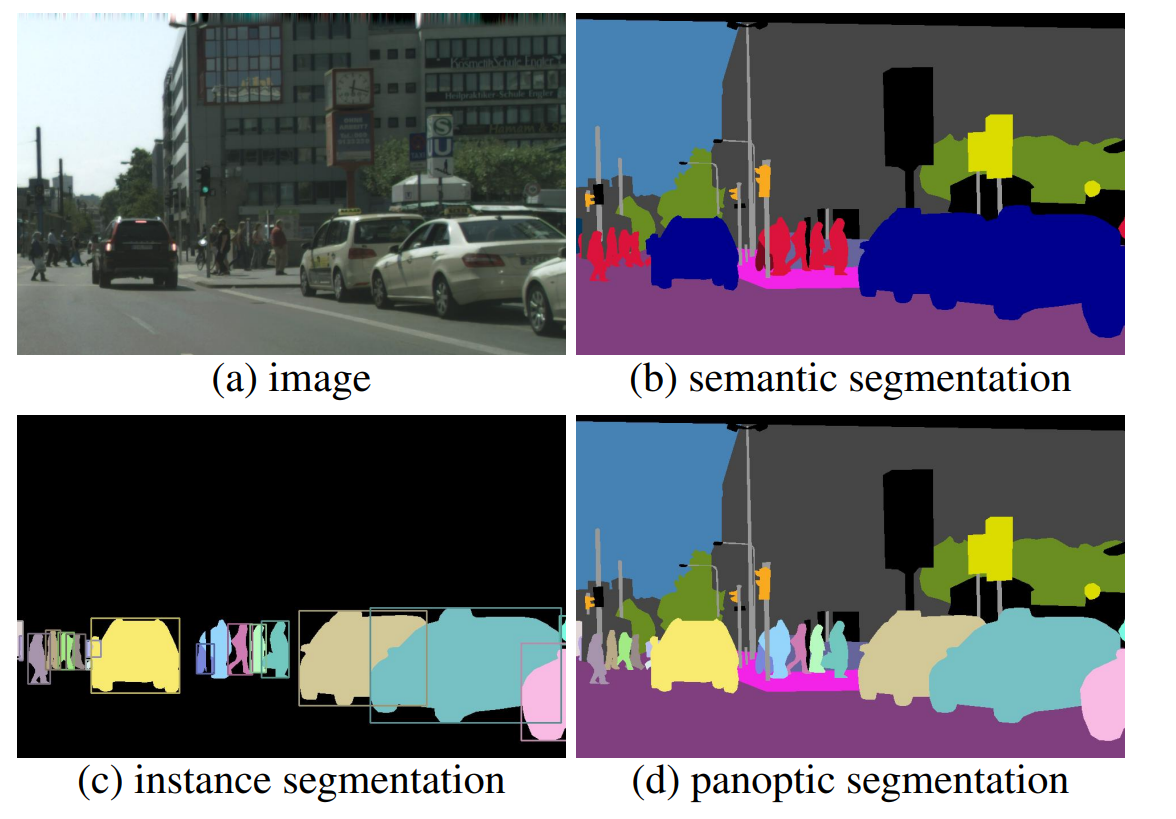
\includegraphics[width=10cm]{figures/segmantations.png} % leia abaixo
	\legend{Fonte: \citeonline{kirillov2019panoptic}}
	\label{fig:segentacoes}
\end{figure}

\subsubsection*{Segmentação semântica}

A segmentação semântica começou a ter resultados satisfatórios a partir de redes totalmente convolucionais, com o objetivo de segmentar imagens classificando pixels, esse modelo descarta a camada totalmente conectada pois a saída deverá ser uma imagem e não uma classificação — isso a torna mais rápida para treinar do que as redes neurais convolucionais —, logo usa camadas deconvolucionais para transformar a matriz de características em uma imagem de qualquer dimensão na saída. A RTC criou a arquitetura chamada de salto (ou conexões) que serve para evitar perdas em camadas de agrupamento criando conexões entre camadas não consecutivas — geralmente entre camadas convolucionais e deconvolucionais — como apresentado na \cref{fig:rtc}, a arquitetura de salto evoluiu para arquitetura codificador-decodificador.
\begin{figure}[H]
	\caption{Exeplo de arquitetura de rede totalmente convolucional}
	\centering % para centralizarmos a figura
	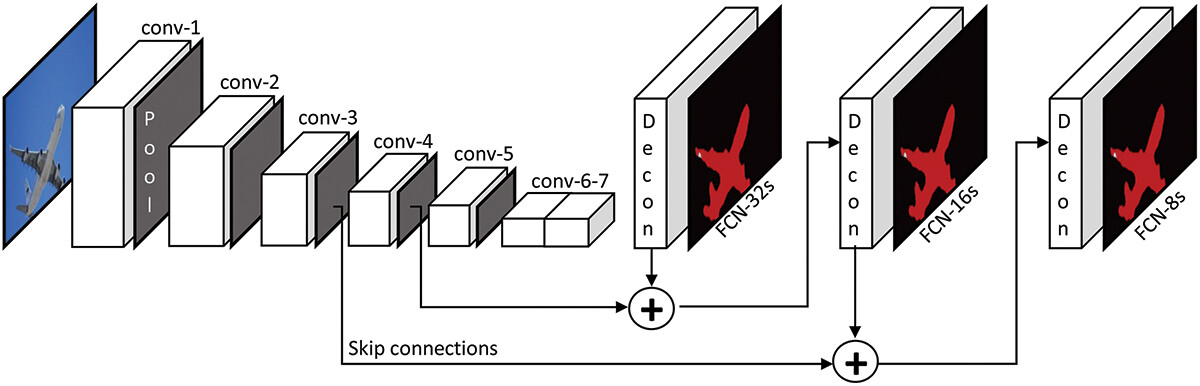
\includegraphics[width=10cm]{figures/redes_totalmente_convolucionais.jpeg} % leia abaixo
	\legend{Fonte: \citeonline{dp_semantic_segmantation}}
	\label{fig:rtc}
\end{figure}

A arquitetura codificador-decodificador — ou Encoder-Decoder —, é separada em dois passos: o primeiro para convergir no mapa de características — chamado de codificador — e o segundo para reverter — chamado de decodificador — as camadas de agrupamento para aumentar a dimensão da saída, usando camadas deconvolucionais e de desagrupamento, outra característica importante é a conexão entre camadas de mesmo nível, como por exemplo a arquitetura UNet que foi a primeira a implementar o padrão Codificador-Decodificador. Na \cref{fig:unet} podemos observar que tem formato da letra U, sendo a descida a parte de codificação e subida decodificação \cite{dp_semantic_segmantation, lapix, unetArq}.

\begin{figure}[H]
	\caption{Arquitetura codificador-decodificador UNet}
	\centering % para centralizarmos a figura
	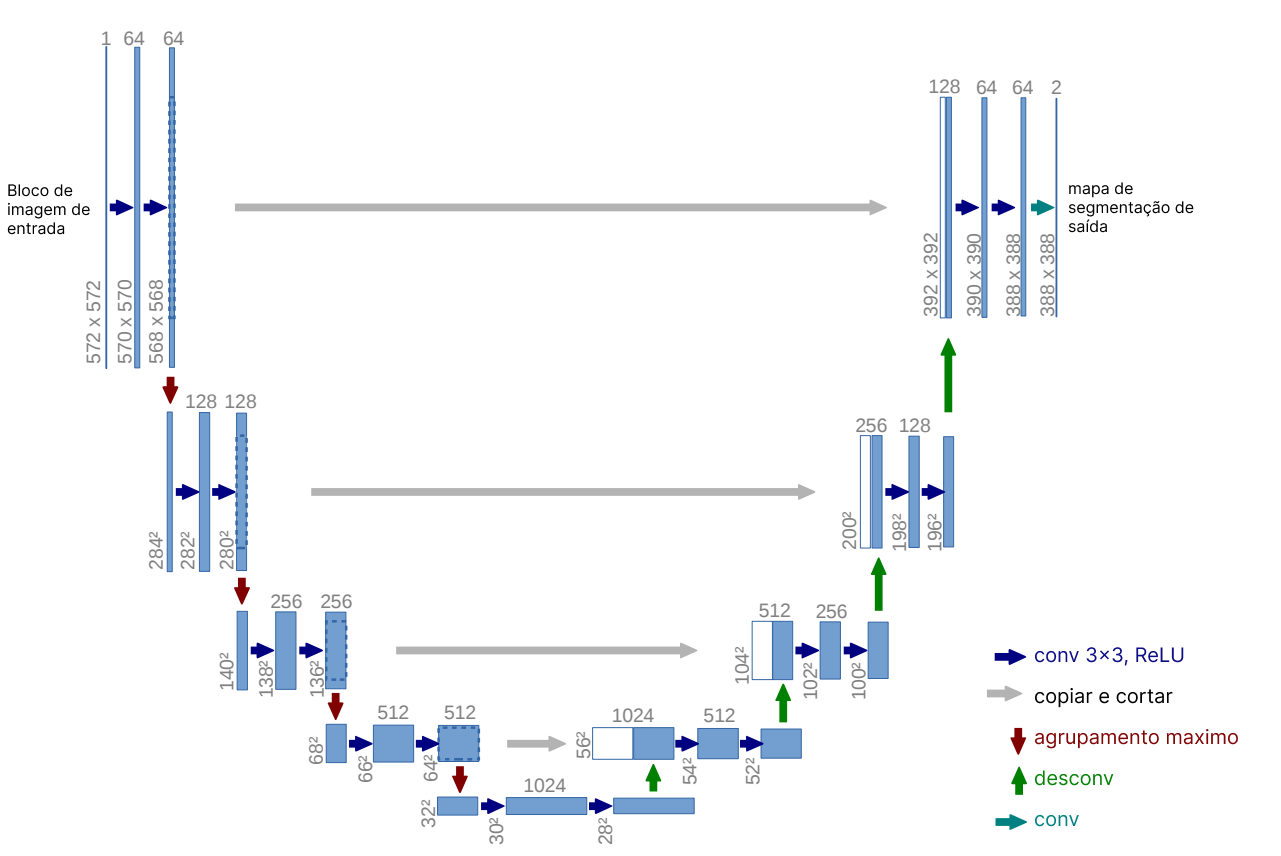
\includegraphics[width=10cm]{figures/unet.png} % leia abaixo
	\legend{Fonte: \citeonline{unetArq}}
	\label{fig:unet}
\end{figure}

\subsubsection*{Segmentação de instância}

Outro problema dentro da área de visão computacional é a detecção de objetos, a primeira solução foi com Características de regiões com RNC — Regions with CNN features (R-CNN) — que se resume em dividir a imagem de entrada em regiões de interesse e nessas regiões aplicar uma RNC. A arquitetura que seleciona essas regiões é chamada de Rede de proposta de região — ou Region Proposal Network (RPN) — o que auxilia na detecção por caixas delimitadoras. Essa ideia inicial foi extendida para segmentação de instância criando também máscara nos objetos, como por exemplo a arquitetura Mask R-CNN \cite{dp_semantic_segmantation, lapix}.

A arquitetura Mask R-CNN é derivado do Fast R-CNN — aprimoramento do R-CNN aplicando conceito RoIPool para classificar — onde há uma segmentação de máscara em cada RoI — ou Região de interresse — paralela com a classificação da caixa delimitadora. A máscara é classificada com uma pequena FCN — ou rede totalmente convolucional — em cada RoI. Além de ter uma pequena melhoria na RoIPool, pois havia um problema de alinhamento nas localizações espaciais exatas, essa camada é chamada de RoIAlign \cite{maskRCNN}.

\subsubsection*{Segmentação panóptica}

Um problema encontrado na segmentação semântica é que objetos de mesma classe não são separados igual na segmentação de instância, logo surgiu uma ideia para criar uma solução usando as duas técnicas. Esse conceito surgiu do trabalho \citeonline{kirillov2019panoptic} e consiste na definição geral da ideia, uma métrica — que será explicada posteriormente — unificada para classificar os resultados do modelo além de fazer a distinção entre coisas — ou stuff — que não são contáveis, como o céu e os objetos — ou things — que são contáveis como carros, pessoas, etc.

\subsubsection*{Modelo escolhido}

Com base no contexto acima percebemos que a segmentação panóptica é a mais completa e por efeito de estudos utilizaremos o mesmo para concluir o trabalho. Como nesse nicho existem várias alternativas abordaremos algumas métricas, técnicas e resultados para selecionar o modelo.

\subsubsubsection*{União sobre intersecção}

A união sobre intersecção — Intersection over Union (IoU) — ou índice de Jaccard é uma métrica muito utlizada para calcular a eficiência de modelos de segmentação, ela se baseia em encontrar uma relação entre a área das classes da imagem de saída com as classes na imagem do conjunto de dados, segue a fôrmula \cite{dp_semantic_segmantation, lapix, kirillov2019panoptic}:

$$ 
IoU = \frac{\text{Área de intersecção}}{\text{Área de união}} \quad IoU(p_i, g) = \frac{p_i \cap g}{ p_i \cup g}
$$

\subsubsubsection*{Classificação de conjuntos}

A classificação de conjuntos é uma técnica para criar relações entre a imagem de predição e a imagem do conjunto de dados. Ela se divide em três classificações sendo elas: Positivos Verdadeiros — ou True Positives(TP) — sendo o requisito ter uma intersecção significativa entre classes iguais, \emph{i.e.}, IoU > 0.5, Falso Positivos — ou False Positives(FP) — quando um objeto não é correspondido na imagem de predição e por fim Falso Negativos — False Negatives(FN) — quando um objeto não é correspondido na imagem do conjunto de dados, podemos obsevar esses conceitos de conjuntos na \cref{fig:conjuntos} \cite{kirillov2019panoptic}.
\begin{figure}[H]
	\caption{Exeplo da classificação dos conjuntos usados nas métricas de segmentação}
	\centering % para centralizarmos a figura
	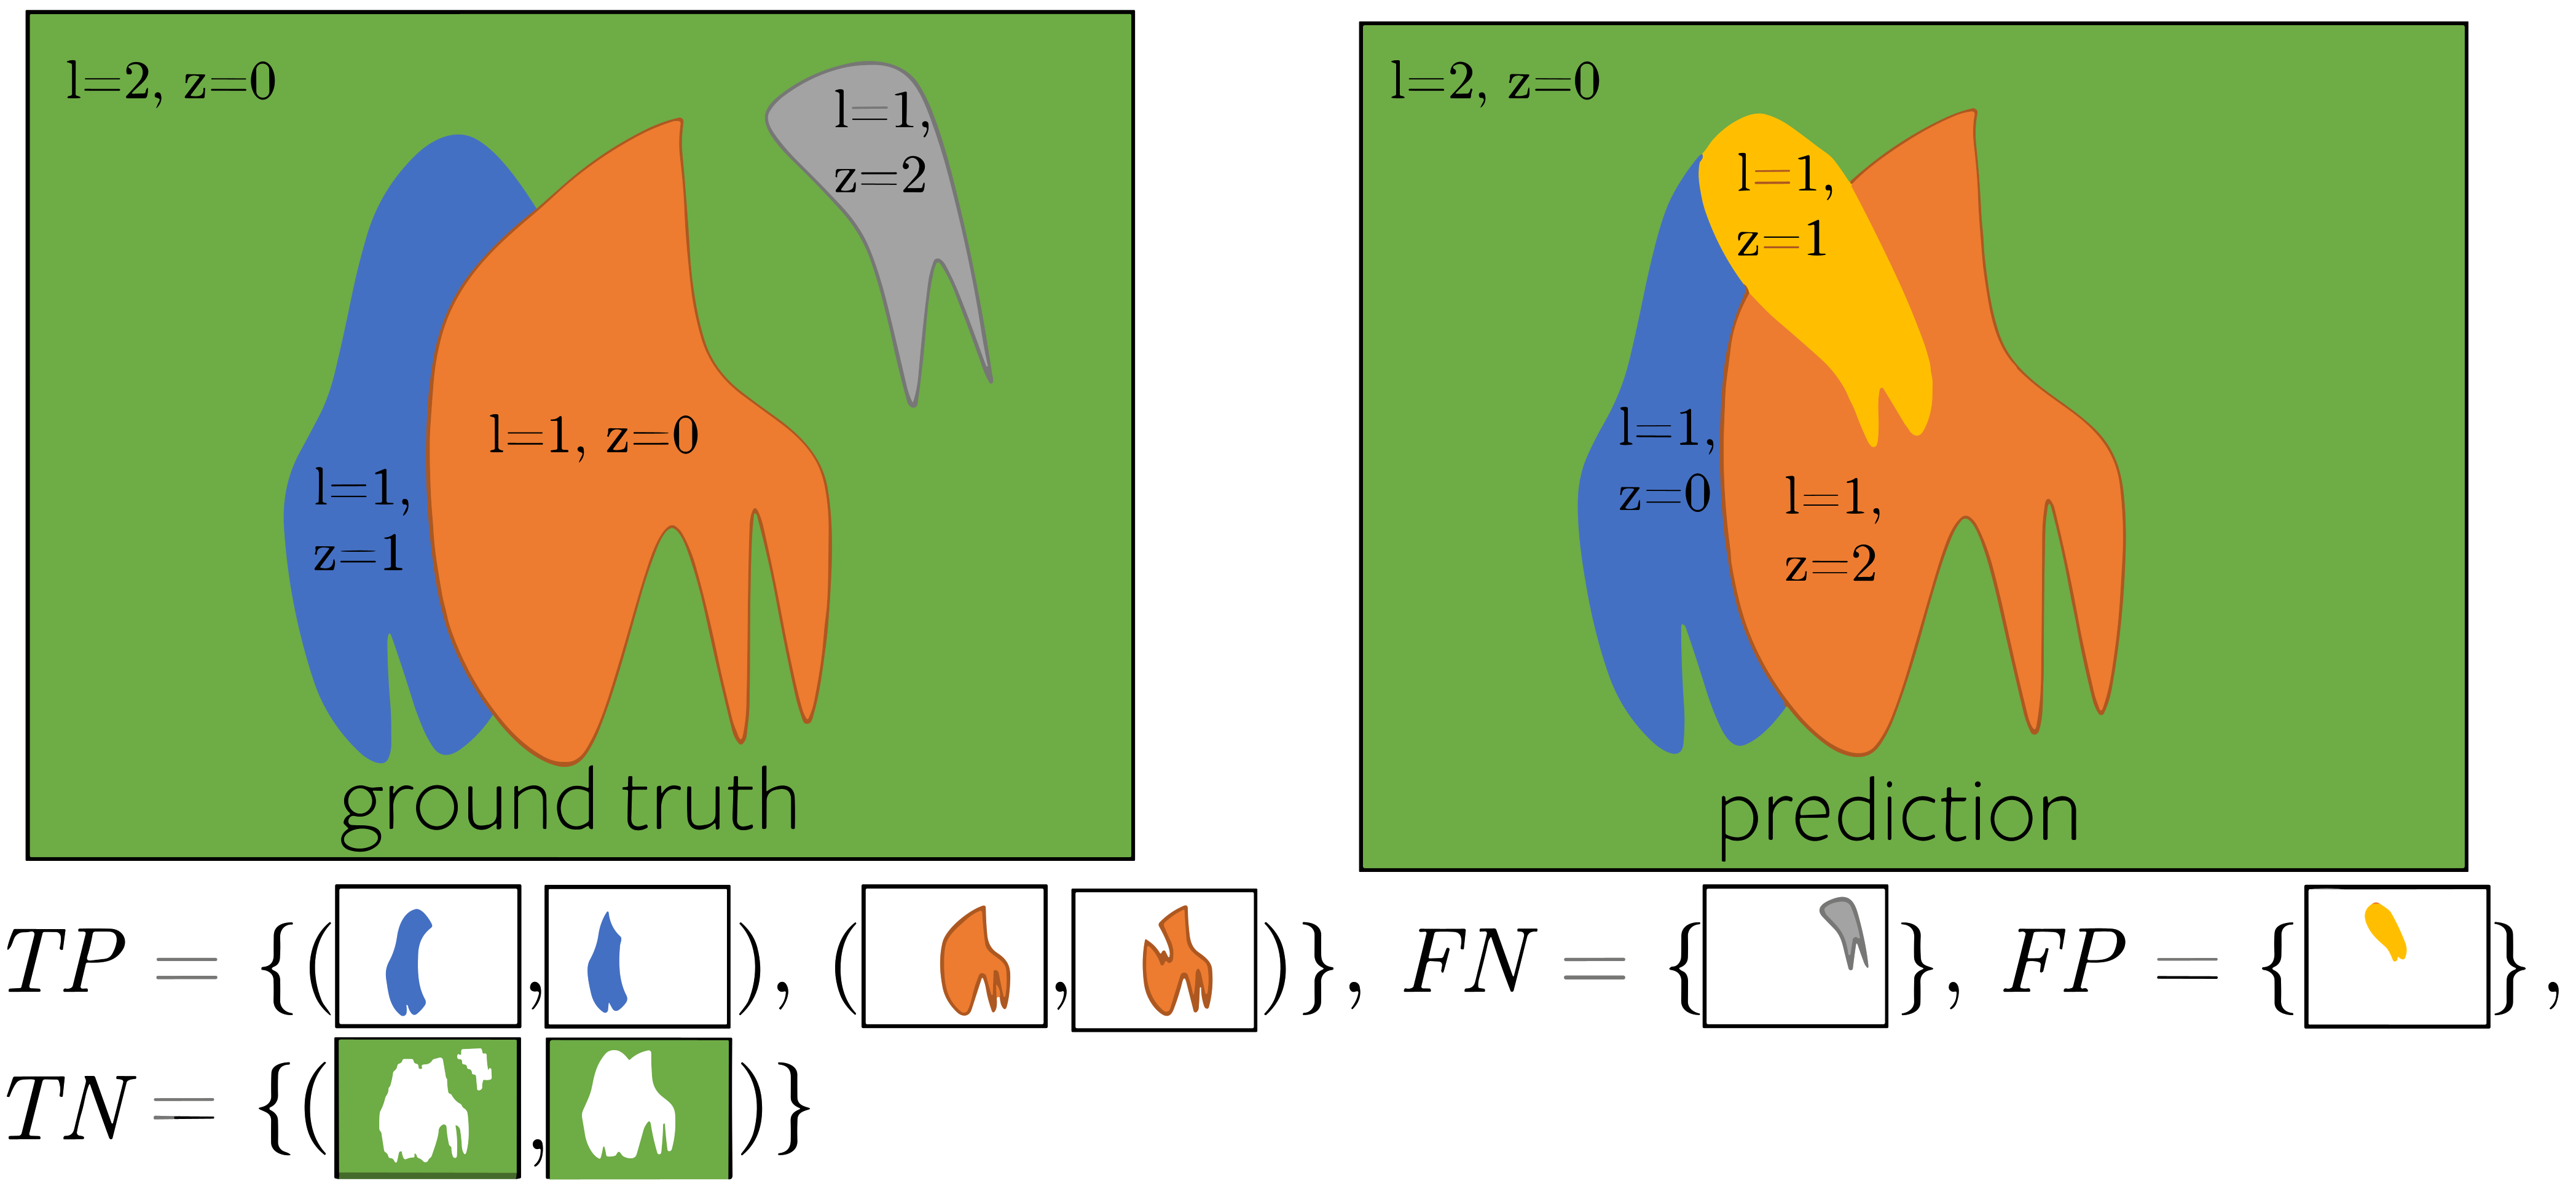
\includegraphics[width=10cm]{figures/pan_metric.png} % leia abaixo
	\legend{Fonte: \citeonline{slidesKirillov}}
	\label{fig:conjuntos}
\end{figure}

\subsubsubsection*{Qualidade panóptica}

A qualidade panóptica — ou Panoptic Quality (PQ) — foi definido pela primeira vez no artigo \citeonline{kirillov2019panoptic}, e se resume na formula:

\begin{equation}
\label{eq:pq_metric}
PQ = \frac{\sum_{(p,g)\in TP}IoU(p,g)}{ |TP| + \frac{1}{2}|FP| + \frac{1}{2}|FN|}
\end{equation}

Multiplicando a \cref{eq:pq_metric} por $\frac{|TP|}{|TP|}$ temos:

\begin{equation*}
	PQ = \underbrace{\frac{\sum_{(p,g)\in TP}IoU(p,g)}{|TP|}}_{\text{Segmentation Quality (SQ)}} 
	\times
	\underbrace{\frac{|TP|}{|TP| + \frac{1}{2}|FP| + \frac{1}{2}|FN|}}_{\text{Recognition Quality (RQ)}}
\end{equation*}

Portanto podemos concluir que PQ é apenas uma simplificação para uma fôrmula que contém uma relação entre métricas de segmentação semântica e de instância.

\subsubsubsection*{Resultados}

Os resultados são de uma competição em aberto criada pela Cytyscapes Dataset, essa competição tem várias modalidades e esses são referentes ao nicho de segmentação panóptica utilizando a métrica PG na classe de pessoas \cite{datasetResults}.
\begin{table}[H]
	\centering
	\caption{Top 15 modelos que melhor classificam pessoas}
	\label{tab:resultados-cityscapes}
	\begin{tabular}{|l|c|}
	  \hline
	  Nome do modelo & Precisão (\%) \\
	  \hline
	  EfficientPS [Mapillary Vistas] & 61,6 \\
	  EfficientPS [Cityscapes-fine] & 60,9 \\
	  Panoptic-DeepLab w/ SWideRNet [Mapillary Vistas + Pseudo-labels] & 60,6 \\
	  hri\_panoptic & 60,6 \\
	  Naive-Student (iterative semi-supervised learning with Panoptic-DeepLab) & 60,2 \\
	  Panoptic-DeepLab w/ SWideRNet [Mapillary Vistas] & 59,8 \\
	  iFLYTEK-CV & 59,2 \\
	  Panoptic-DeepLab [Mapillary Vistas] & 58,5 \\
	  Panoptic-DeepLab w/ SWideRNet [Cityscapes-fine] & 58,4 \\
	  Seamless Scene Segmentation & 57,7 \\
	  Axial-DeepLab-XL [Mapillary Vistas] & 57,2 \\
	  Unifying Training and Inference for Panoptic Segmentation [COCO] & 56,5 \\
	  kMaX-DeepLab [Cityscapes-fine] & 56 \\
	  Axial-DeepLab-L [Mapillary Vistas] & 55,9 \\
	  TASCNet-enhanced & 55,2 \\
	  \hline
	\end{tabular}
  \end{table}
  
  

